\documentclass[11pt]{article}
\usepackage{amssymb}
\usepackage{amsthm}
\usepackage{enumitem}
\usepackage{amsmath, physics}
\usepackage{bm}
\usepackage{adjustbox}
\usepackage{mathrsfs}
\usepackage{graphicx}
\usepackage{siunitx}
\usepackage[mathscr]{euscript}

\title{\textbf{Solved selected problems of Classical Electrodynamics - Hans Ohanian}}
\author{Franco Zacco}
\date{}

\addtolength{\topmargin}{-3cm}
\addtolength{\textheight}{3cm}

\newcommand{\N}{\mathbb{N}}
\newcommand{\Z}{\mathbb{Z}}
\newcommand{\Q}{\mathbb{Q}}
\newcommand{\R}{\mathbb{R}}
\newcommand{\diam}{\text{diam}}
\newcommand{\cl}{\text{cl}}
\newcommand{\bdry}{\text{bdry}}
\newcommand{\inter}{\text{int}}
\newcommand{\uvi}{\bm{i}}
\newcommand{\uvj}{\bm{j}}
\newcommand{\uvk}{\bm{k}}
\newcommand{\hatx}{\bm{\hat{x}}}
\newcommand{\haty}{\bm{\hat{y}}}
\newcommand{\hatz}{\bm{\hat{z}}}
\newcommand{\hatrho}{\bm{\hat{\rho}}}
\newcommand{\hatphi}{\bm{\hat{\phi}}}
\newcommand{\hatr}{\bm{\hat{r}}}
\newcommand{\hattheta}{\bm{\hat{\theta}}}
\newcommand\numberthis{\addtocounter{equation}{1}\tag{\theequation}}

\theoremstyle{definition}
\newtheorem*{solution*}{Solution}
\renewcommand*{\proofname}{\bf{Solution}}

\begin{document}
\maketitle
\thispagestyle{empty}

\section*{Chapter 3 - The Boundary-Value Problem}

\subsection*{Problems}
\begin{proof}{\textbf{1.}}
    If the olive oil inside a closed tin can has a charge $Q$ then these charges
    will attract charges $-Q$ from the inside side of the tin can because of 
    the electrostatic induction and therefore in the outside of the tin can we
    get a charge $Q$.
\end{proof}

\cleardoublepage
\begin{proof}{\textbf{3.}}
    Let us consider two image charges $-q$ at $(-b, b, 0)$, $(b, -b, 0)$ and 
    another image charge $q$ at $(-b, -b, 0)$ then the potential equation due
    to this charges is 
    \begin{align*}
        \Phi(\bm{x}) &= \frac{q}{\sqrt{(x-b)^2 + (y-b)^2 + z^2}}
        - \frac{q}{\sqrt{(x-b)^2 + (y+b)^2 + z^2}}\\
        &\quad - \frac{q}{\sqrt{(x+b)^2 + (y-b)^2 + z^2}}
        + \frac{q}{\sqrt{(x+b)^2 + (y+b)^2 + z^2}}
    \end{align*}
    We see that if $x = 0$ we have that 
    \begin{align*}
        \Phi((0,y,z)) &= \frac{q}{\sqrt{(-b)^2 + (y-b)^2 + z^2}}
        - \frac{q}{\sqrt{(-b)^2 + (y+b)^2 + z^2}}\\
        &\quad - \frac{q}{\sqrt{(b)^2 + (y-b)^2 + z^2}}
        + \frac{q}{\sqrt{(b)^2 + (y+b)^2 + z^2}}\\
        &= 0
    \end{align*}
    And if $y = 0$ we get that
    \begin{align*}
        \Phi((x,0,z)) &= \frac{q}{\sqrt{(x-b)^2 + (-b)^2 + z^2}}
        - \frac{q}{\sqrt{(x-b)^2 + (b)^2 + z^2}}\\
        &\quad - \frac{q}{\sqrt{(x+b)^2 + (-b)^2 + z^2}}
        + \frac{q}{\sqrt{(x+b)^2 + (b)^2 + z^2}}\\
        &= 0 
    \end{align*}
    Therefore these image charges match the boundary conditions for the
    grounded conducting plates at the $x$-$z$ plane and at the $y$-$z$ plane.
    Hence this equation for $\Phi$ describes the potential at the region
    $x>0$, $y>0$ as we wanted.

    Now, let us compute the electric field components at $(b,b,0)$ as follows
    \begin{align*}
        E_x &= -\pdv{\Phi}{x}\bigg|_{(b,b,0)}\\
        &= q\bigg[\frac{(x-b)}{((x-b)^2 + (y-b)^2 + z^2)^{3/2}}
        - \frac{(x-b)}{((x-b)^2 + (y+b)^2 + z^2)^{3/2}}\\
        &\quad- \frac{(x+b)}{((x+b)^2 + (y-b)^2 + z^2)^{3/2}}
        + \frac{(x+b)}{((x+b)^2 + (y+b)^2 + z^2)^{3/2}}
        \bigg]_{(b,b,0)}\\
        &= q\bigg[- \frac{2b}{((2b)^2)^{3/2}}
        + \frac{2b}{((2b)^2 + (2b)^2)^{3/2}}\bigg]\\
        &= q\bigg[-\frac{1}{4b^2} + \frac{1}{8\sqrt{2}b^2}\bigg]
    \end{align*}
    \begin{align*}
        E_y &= -\pdv{\Phi}{y}\bigg|_{(b,b,0)}\\
        &= q\bigg[\frac{(y-b)}{((x-b)^2 + (y-b)^2 + z^2)^{3/2}}
        - \frac{(y-b)}{((x+b)^2 + (y-b)^2 + z^2)^{3/2}}\\
        &\quad- \frac{(y+b)}{((x-b)^2 + (y+b)^2 + z^2)^{3/2}}
        + \frac{(y+b)}{((x+b)^2 + (y+b)^2 + z^2)^{3/2}}\bigg]_{(b,b,0)}\\
        &= q\bigg[- \frac{2b}{((2b)^2)^{3/2}}
        + \frac{2b}{((2b)^2 + (2b)^2)^{3/2}}\bigg]\\
        &= q\bigg[-\frac{1}{4b^2} + \frac{1}{8\sqrt{2}b^2}\bigg]
    \end{align*}
    \begin{align*}
        E_z &= -\pdv{\Phi}{z}\bigg|_{(b,b,0)}\\
        &= q\bigg[\frac{z}{((x-b)^2 + (y-b)^2 + z^2)^{3/2}}
        - \frac{z}{((x+b)^2 + (y-b)^2 + z^2)^{3/2}}\\
        &\quad- \frac{z}{((x-b)^2 + (y+b)^2 + z^2)^{3/2}}
        + \frac{z}{((x+b)^2 + (y+b)^2 + z^2)^{3/2}}\bigg]_{(b,b,0)}\\
        &= 0
    \end{align*}
    Therefore the force that the conducting plates exert on the point charge
    is
    \begin{align*}
        \bm{F} = q\bm{E}
        = q(E_x\uvi + E_y\uvj)
        = q^2\bigg[-\frac{1}{4b^2} + \frac{1}{8\sqrt{2}b^2}\bigg](\uvi + \uvj)
    \end{align*}
\end{proof}

\cleardoublepage
\begin{proof}{\textbf{4.}}
    Let a point charge $q$ at $x=3a$ and let us consider an image charge $q'$
    at $x = b$ then the potential because of these charges is given by
    \begin{align*}
        \Phi(\bm{x}) &= \frac{q}{\sqrt{(x-3a)^2 + y^2 + z^2}}
        + \frac{q'}{\sqrt{(x-b)^2 + y^2 + z^2}}
    \end{align*}
    Let us take a point $(x,y,z)$ such that $\sqrt{x^2 + y^2 + z^2} = a$ we
    want that $\Phi(x,y,z) = 0$ at this point, then
    \begin{align*}
        0 = \frac{q}{\sqrt{(x-3a)^2 + y^2 + z^2}}
        + \frac{q'}{\sqrt{(x-b)^2 + y^2 + z^2}}\\
        -\frac{q'}{\sqrt{(x-b)^2 + y^2 + z^2}}
        = \frac{q}{\sqrt{(x-3a)^2 + y^2 + z^2}}\\
        \sqrt{\frac{(x-b)^2 + y^2 + z^2}{(x-3a)^2 + y^2 + z^2}}
        = -\frac{q'}{q}\\
        \frac{x^2 - 2bx + b^2 + y^2 + z^2}{x^2 -6ax + 9a^2 + y^2 + z^2}
        = \left(\frac{q'}{q}\right)^2\\
        \frac{a^2 - 2bx + b^2}{a^2 -6ax + 9a^2}
        = \left(\frac{q'}{q}\right)^2\\
        \frac{a^2 - 2bx + b^2}{10a^2 -6ax}
        = \left(\frac{q'}{q}\right)^2\\
        b^2 - 2bx + a^2 - \left(\frac{q'}{q}\right)^2(10a^2 -6ax) = 0\\
        x\left(6a\left(\frac{q'}{q}\right)^2 - 2b\right)
        + \left(b^2  + a^2 - 10a^2\left(\frac{q'}{q}\right)^2\right) = 0
    \end{align*}
    This equation is satisfied if 
    \begin{align*}
        6a\left(\frac{q'}{q}\right)^2 - 2b = 0\\
        b^2  + a^2 - 10a^2\left(\frac{q'}{q}\right)^2 = 0
    \end{align*}
    So $\left(\frac{q'}{q}\right)^2 = \frac{b}{3a}$ and replacing we have that
    \begin{align*}
        b^2 - \frac{10}{3}ab + a^2 = 0
    \end{align*}
    For which we have that $b = a/3$ and $b = 3a$ are solutions.
    Using that $b = a/3$ we get that 
    \begin{align*}
        q' = \pm\frac{q}{3}
    \end{align*}
    Because if we set $b = 3a$ then we get that $q' = \pm q$ for which we will
    get that $\Phi(\bm{x}) = 0$ which is a trivial solution.
    Therefore the potential at any point is given by
    \begin{align*}
        \Phi(\bm{x}) &= \frac{q}{\sqrt{(x-3a)^2 + y^2 + z^2}}
        - \frac{q}{3\sqrt{(x-a/3)^2 + y^2 + z^2}}
    \end{align*}
    Where we have taken the negative solution for $q'$.
    Let us write the result as a function of the spherical coordinates
    $r, \alpha$ as follows
    \begin{align*}
        \Phi(\bm{x}) &= \frac{q}{\sqrt{x^2 - 6ax + 9a^2 + y^2 + z^2}}
        - \frac{q}{3\sqrt{x^2 -2ax/3 + a^2/9 + y^2 + z^2}}\\
        &= \frac{q}{\sqrt{r^2 - 6ar\cos\alpha + 9a^2}}
        - \frac{q}{3\sqrt{r^2 -(2/3)ar\cos\alpha + a^2/9}}
    \end{align*}
    Where we used that $x = r\cos\alpha$.

    On the other hand, we know that the magnitude of the electric field just
    outside a conductor is proportional to the local surface charge density 
    on the conductor $E_{ext} = 4\pi \sigma$.

    Then, let us determine the $r$ component of the electric field $E$ at
    $(a, \alpha, \theta)$ as follows
    \begin{align*}
        E_r &= -\pdv{\Phi}{r}\bigg|_{(a, \alpha, \theta)}\\
        &= q\bigg[
            \frac{9r - 3a\cos\alpha}{(a^2 - 6ar\cos\alpha + 9r^2)^{3/2}}
            + \frac{3a\cos\alpha - r}{(9a^2 - 6ar\cos\alpha + r^2)^{3/2}}
        \bigg]_{(a, \alpha, \theta)}\\
        &= q\bigg[
            \frac{9a - 3a\cos\alpha}{(a^2 - 6a^2\cos\alpha + 9a^2)^{3/2}}
            - \frac{a - 3a\cos\alpha}{(9a^2 - 6a^2\cos\alpha + a^2)^{3/2}}
        \bigg]\\
        &= q\bigg[
            \frac{a(9 - 3\cos\alpha)}{a^3(10 - 6\cos\alpha)^{3/2}}
            - \frac{a(1 - 3\cos\alpha)}{a^3(10 - 6\cos\alpha)^{3/2}}
        \bigg]\\
        &= q\bigg[
            \frac{9 - 3\cos\alpha - 1 + 3\cos\alpha}{a^2(10 - 6\cos\alpha)^{3/2}}
        \bigg]\\
        &= \frac{8q}{a^2(10 - 6\cos\alpha)^{3/2}}
    \end{align*}
    Then since $E_r|_{(a, \alpha, \theta)} = 4\pi \sigma$ we get that
    \begin{align*}
        \sigma &= \frac{q}{4\pi a^2}\frac{8}{(10 - 6\cos\alpha)^{3/2}}
    \end{align*}    
\end{proof}

\cleardoublepage
\begin{proof}{\textbf{5.}}
    Let the two infinite conducting plates be at $x=\pm d$ and the point charge
    at the origin. Also, let us consider an infinite sequence of image charges
    where they alternate their charge between $\pm q$ and they are placed at
    $x = 2d, -2d, 4d, -4d, ...$, then the potential is given by
    \begin{align*}
        \Phi(\bm{x}) = \frac{q}{\sqrt{x^2+y^2 + z^2}}
        + \sum_{n=1}^\infty \frac{(-1)^nq}{\sqrt{(x- 2dn)^2 + y^2 + z^2}}
        + \frac{(-1)^nq}{\sqrt{(x + 2dn)^2 + y^2 + z^2}}
    \end{align*}
    So if we consider $x=\pm d$ for any value of $y$ and $z$ the equation
    converges to 0 as it should for the grounded plates.
    \begin{align*}
        \Phi(\bm{x}) = \frac{q}{\sqrt{d^2+y^2 + z^2}}
        - \frac{q}{\sqrt{d^2 + y^2 + z^2}} = 0
    \end{align*}
\end{proof}

\cleardoublepage
\begin{proof}{\textbf{7.}}
    The electrostatic potential generated by a point charge placed at a
    distance $b$ from a very large conducting plate is 
    \begin{align*}
        \Phi(\bm{x}) = \frac{q}{\sqrt{x^2 + y^2 + (z - b)^2}}
        - \frac{q}{\sqrt{x^2 + y^2 + (z + b)^2}}
    \end{align*}
\begin{itemize}
    \item [(a)] The perpendicular component of the electric field to the
    conducting plate is $E_z$. Let us compute $E_z$ at $(x, y, 0)$ as follows 
    \begin{align*}
        E_z &= -\pdv{\Phi}{z}\bigg|_{(x, y, 0)}\\
        &= q\bigg[
            \frac{(z - b)}{(x^2 + y^2 + (z - b)^2)^{3/2}}
            - \frac{(z + b)}{(x^2 + y^2 + (z + b)^2)^{3/2}}
        \bigg]_{(x, y, 0)}\\
        &= -\frac{2qb}{(x^2 + y^2 + b^2)^{3/2}}
    \end{align*}
    But since $E_{\perp} = E_z = 4\pi\sigma$ we get that the surface charge
    density on the plate is
    \begin{align*}
        \sigma &= -\frac{qb}{2\pi(x^2 + y^2 + b^2)^{3/2}}
    \end{align*}
    \item [(b)] The electric field $\bm{E}$ at the plate is $\bm{E}$ valued at
    $(x,y,0)$. We found the $z$ component of $\bm{E}$ in part (a) at this point
    hence the components $x$ and $y$ are
    \begin{align*}
        E_x &= -\pdv{\Phi}{x}\bigg|_{(x, y, 0)}\\
        &= q\bigg[
            \frac{x}{(x^2 + y^2 + (z - b)^2)^{3/2}}
            - \frac{x}{(x^2 + y^2 + (z + b)^2)^{3/2}}
        \bigg]_{(x, y, 0)}\\
        &= 0\\
        E_y &= -\pdv{\Phi}{y}\bigg|_{(x, y, 0)}\\
        &= q\bigg[
            \frac{y}{(x^2 + y^2 + (z - b)^2)^{3/2}}
            - \frac{y}{(x^2 + y^2 + (z + b)^2)^{3/2}}
        \bigg]_{(x, y, 0)}\\
        &= 0
    \end{align*}
    This result makes sense since by symmetry the components $E_x$ and $E_y$
    cancel out. Therefore $\bm{E}$ at $(x,y,0)$ is 
    \begin{align*}
        \bm{E}|_{(x,y,0)} &= \begin{pmatrix}
            0 \\ 0 \\ -\frac{2qb}{(x^2 + y^2 + b^2)^{3/2}}
        \end{pmatrix}
    \end{align*}
\cleardoublepage
    \item [(c)] Given that the components $E_x$ and $E_y$ of the electric field
    are $0$ at the plate the force per unit of area has one component in the
    $z$ direction given by
    \begin{align*}
        f_z = 2\pi \sigma^2
    \end{align*}
    Since $2\pi\sigma$ is the electric field at the plate without the
    contribution of the local surface charge of the plate.
    Then by integration we can get the total force over the entire plate as
    follows
    \begin{align*}
        F_z &= 2\pi \int_{-\infty}^\infty\int_{-\infty}^\infty
        \frac{q^2b^2}{4\pi^2(x^2 + y^2 + b^2)^3}~dxdy\\
        &= \frac{q^2b^2}{2\pi}\int_{-\infty}^\infty\int_{-\infty}^\infty
        \frac{1}{(x^2 + y^2 + b^2)^3}~dxdy\\
        &= \frac{q^2b^2}{2\pi}\int_{-\infty}^\infty
        \frac{3\pi}{8(y^2 + b^2)^{5/2}}~dy\\
        &= \frac{3q^2b^2}{16}\frac{4}{3b^4}\\
        &= \frac{q^2}{4b^2}
    \end{align*}
    Which is exactly the same force the plate exerts on the charge.
\end{itemize}
\end{proof}

\cleardoublepage
\begin{proof}{\textbf{8.}}
\begin{itemize}
    \item [(a)] The work needed to remove the point charge from the distance $b$
    to infinity is
    \begin{align*}
        W &= \int_{b}^\infty F_z ~dz\\
        &= \int_b^\infty \frac{q^2}{4z^2}~dz\\
        &= \frac{q^2}{4}\bigg[-\frac{1}{z}\bigg]_b^\infty\\
        &= \frac{q^2}{4b}
    \end{align*}
    Where we integrated over $z$ (previously named $b$) since now it is a variable
    as the charge moves.

    The mutual potential energy between the charge and the (virtual) image
    charge is
    \begin{align*}
        U = \frac{q^2}{2b}
    \end{align*}
    Since they are separated a distance $2b$. Therefore the mutual potential
    energy does not agree with the work.
    \item [(b)] To take a charge from a distance $b$ to the plate, to
    infinity, we need to do a work $W =q^2/4b$ (gaining potential energy)
    then to bring the charge form infinity to a distance
    $b$ of the conducting plate the charge must convert the same potential
    energy gained to kinetic energy. Therefore the kinetic energy at
    $b = 10 \mathring{A}$ is 
    \begin{align*}
        K &= \frac{(1.602\times 10^{-19})^2}{4(10^{-10})} \frac{C^2}{m}\\
        &= 6.416 \times 10^{-30} \frac{C^2}{m} \cdot
        \frac{1}{4\pi\epsilon_0} \frac{Nm^2}{C^2}\\
        &= 5.766 \times 10^{-20}~J \cdot \\
        &= 5.766 \times 10^{-20}~J \frac{1~eV}{1.602 \times 10^{-19}~J}\\
        &= 0.36~eV
    \end{align*}
\end{itemize}
\end{proof}

\cleardoublepage
\begin{proof}{\textbf{9.}}
    From equation (29) we know that the solution to Laplace's equation in
    rectangular coordinates is of the form 
    $$\Phi(x,y,z) = e^{\pm\alpha x}e^{\pm\beta y}e^{\pm\gamma z}$$
    multiplied by some arbitrary constant.\\
    By comparison with the boundary conditions must be that the $X(x)$ function
    is $X(x) = \sin(4x)$ and the $Y(y)$ function is $Y(y) = \cos(3y)$
    which can be written as a combination of exponentials.\\
    To determine $Z(z)$ we first see that $\pm\alpha = \pm 4i$ and
    $\pm\beta = \pm 3i$ since
    \begin{align*}
        \sin(4x) = \frac{1}{2i}(e^{4ix} - e^{-4ix})\\
        \cos(3y) = \frac{1}{2}(e^{3iy} + e^{-3iy})
    \end{align*}
    Then using the relation
    \begin{align*}
        \alpha^2 + \beta^2 + \gamma^2 = 0
    \end{align*}
    We can get $\pm\gamma$ as follows
    \begin{align*}
        \pm\gamma &= \pm\sqrt{-\alpha^2 - \beta^2}
        = \pm\sqrt{-(\pm 4i)^2 - (\pm 3i)^2}
        = \pm\sqrt{16 + 9} = \pm 5
    \end{align*}
    Then $Z(z) = e^{\pm5z}$. So $\Phi(x,y,z)$ is given by
    \begin{align*}
        \Phi(x,y,z) = (Ae^{5z} + Be^{-5z}) \sin(4x)\cos(3y)
    \end{align*}
    We can determine the constants $A$ and $B$ using the boundary conditions.
    We see that
    \begin{align*}
        \Phi(x,y,0) &= (A + B)\sin(4x)\cos(3y) = 5\sin(4x)\cos(3y)\\
        \Phi(x,y,2/5) &= (Ae^2 + Be^{-2})\sin(4x)\cos(3y) = 2\sin(4x)\cos(3y)
    \end{align*}
    So $A = 5 - B$ from the first boundary condition and hence from the second
    \begin{align*}
        (5-B)e^2 + Be^{-2} &= 2\\
        B (e^{-2} - e^2) &= 2 - 5e^2\\
        B &= \frac{2 - 5e^2}{e^{-2} - e^2}
    \end{align*}
    Therefore
    \begin{align*}
        \Phi(x,y,z)
        = \bigg(5e^{5z} + \frac{2 - 5e^2}{e^{-2} - e^2}(e^{-5z}- e^{5z})\bigg)
        \sin(4x)\cos(3y)
    \end{align*}
\end{proof}

\cleardoublepage
\begin{proof}{\textbf{10.}}
Let us consider our cube to be
\begin{center}
    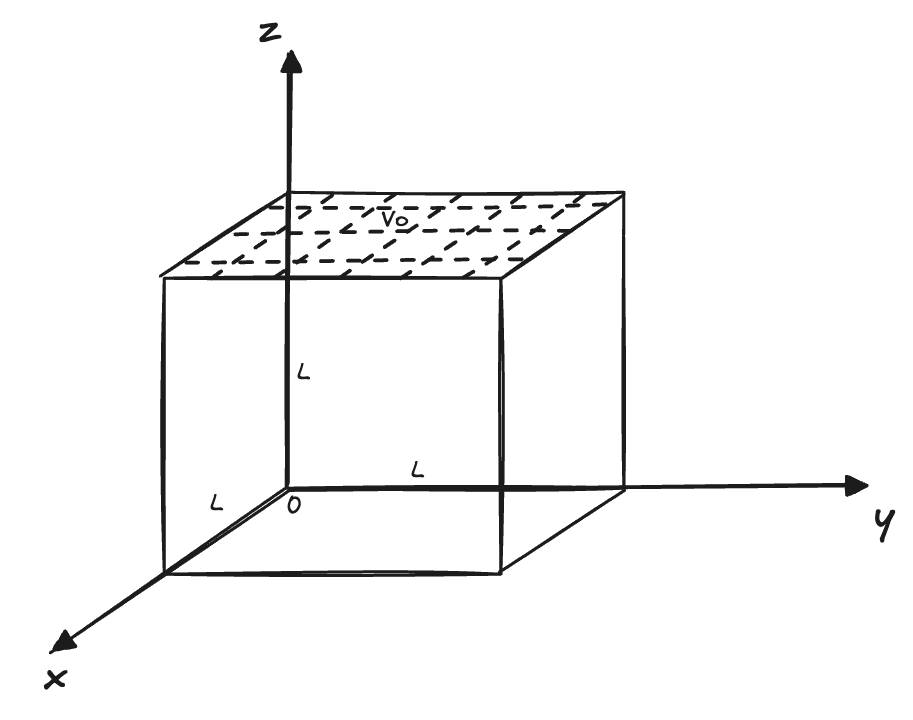
\includegraphics[scale=0.3]{ch3-10.png}
\end{center}
Then the following boundary conditions must hold
\begin{align*}
    \Phi(0, y, z) &= 0 \quad \Phi(x, 0, z) = 0 \quad \Phi(x, y, 0) = 0\\
    \Phi(L, y, z) &= 0 \quad \Phi(x, L, z) = 0 \quad \Phi(x, y, L) = V_0
\end{align*}
Let us consider the $X(x)$ function of $\Phi$, we see that $\Phi$ must vanish
when $x = 0$ and $x = L$ then we can take this function to be
$X(x) = \sin(\pi x/L)$, in the same way since $\Phi$ must vanish when $y=0$
and when $y = L$ we can take $Y(y) = \sin(\pi y/L)$. But in this way the
funcitons of $\Phi$ will have values outside the cube, so we must take a
combination of them as follows
\begin{align*}
    \Phi(x,y,z) = \sum_{n,m=-\infty}^{n,m=\infty}
    A_{nm}\sin(\frac{\pi n x}{L}) \sin(\frac{\pi m y}{L})e^{\pm\gamma_{nm} z}
\end{align*}
Given that the term where $n = m = 0$ is zero and the negative terms can be
combined with the positive terms we can write the sum between $n, m = 1$ to
infinity i.e.
\begin{align*}
    \Phi(x,y,z) = \sum_{n,m=1}^{n,m=\infty}
    A_{nm}\sin(\frac{\pi n x}{L}) \sin(\frac{\pi m y}{L})e^{\pm\gamma z}
\end{align*}
We know also that $\alpha^2 + \beta^2 + \gamma^2 = 0$ so $\gamma$ must be 
\begin{align*}
    \bigg(\pm\frac{\pi i n}{L}\bigg)^2 &+ \bigg(\pm\frac{\pi i m}{L}\bigg)^2
    + \gamma^2 = 0\\
    \gamma^2 &= \frac{\pi^2 n^2}{L^2} + \frac{\pi^2m^2}{L^2}\\
    \gamma &= \pm\frac{\pi}{L}\sqrt{n^2 + m^2}
\end{align*}
Then the function $Z(z)$ is of the form
$$Ae^{\frac{\pi z}{L}\sqrt{n^2 + m^2}} + Be^{-\frac{\pi z}{L}\sqrt{n^2 + m^2}}$$
From the boundary conditions $\Phi = 0$ when $z = 0$ and $\Phi = V_0$ when
$z = L$ we can determine the values of $A$ and $B$. From the first boundary
condition we get that $B = -A$ hence from the second boundary condition
we get that
\begin{align*}
    Ae^{\pi\sqrt{n^2 + m^2}} &- Ae^{-\pi\sqrt{n^2 + m^2}} = V_0\\
    A(e^{\pi\sqrt{n^2 + m^2}} &- e^{-\pi\sqrt{n^2 + m^2}}) = V_0\\
    A &= \frac{V_0}{e^{\pi\sqrt{n^2 + m^2}} - e^{-\pi\sqrt{n^2 + m^2}}}
\end{align*}
Then the function $Z(z)$ becomes 
\begin{align*}
    \frac{V_0(e^{\frac{\pi z}{L}\sqrt{n^2 + m^2}} - e^{-\frac{\pi z}{L}\sqrt{n^2 + m^2}})}
    {e^{\pi\sqrt{n^2 + m^2}} - e^{-\pi\sqrt{n^2 + m^2}}}
\end{align*}
But multiplying numerator and denominator by $1/2$ we get that
\begin{align*}
    \frac{V_0\sinh(\frac{\pi z}{L}\sqrt{n^2 + m^2})}{\sinh(\pi\sqrt{n^2 + m^2})}
\end{align*}
Finally, to determine $A_{nm}$, let us multiply $\Phi(x,y,L)$ by
$\sin(\frac{\pi n'x}{L}) \sin(\frac{\pi m'y}{L})$ where $n', m' \in \N$.
Let us also integrate with respect to $x$ and $y$ from $0$ to $L$ then
\begin{align*}
    &\int_0^L\int_0^L\Phi(x,y,L)\sin(\frac{\pi n' x}{L}) \sin(\frac{\pi m' y}{L})~dxdy\\
    &\qquad= V_0\sum_{n,m=1}^{n,m=\infty}
    A_{nm}\int_0^L\int_0^L \sin(\frac{\pi n x}{L})
    \sin(\frac{\pi m y}{L})\sin(\frac{\pi n' x}{L}) \sin(\frac{\pi m' y}{L})~dxdy
\end{align*}
Analyzing the integral of the right-hand side we see that
\begin{align*}
    \int_0^L \sin(\frac{\pi n x}{L})\sin(\frac{\pi n' x}{L})~dxdy
    = \begin{cases}
        0 &\text{ if } n \neq n'\\
        L/2 &\text{ if }n = n'
    \end{cases}
\end{align*}
So the only non-zero term on the right side is for $n'$ and $m'$, then
the right-hand side is $V_0A_{n'm'}L^2/4$.
Then, noting that $\Phi(x, y, L) = V_0$ we get that
\begin{align*}
    \frac{V_0L^2}{4} A_{n'm'} &= V_0
    \int_0^L\int_0^L\sin(\frac{\pi n' x}{L}) \sin(\frac{\pi m' y}{L})~dxdy\\
    A_{n'm'} &= \frac{4}{L^2}
    \int_0^L\int_0^L\sin(\frac{\pi n' x}{L}) \sin(\frac{\pi m' y}{L})~dxdy\\
    A_{n'm'} &= \frac{4}{L^2}
    \frac{4L^2\sin^2(\frac{\pi n'}{2}) \sin^2(\frac{\pi m'}{2})}{\pi^2 m'n'}\\
    A_{n'm'} &= \frac{4[1 - \cos(\pi n')][1 - \cos(\pi m')]}{\pi^2 m'n'}\\
    A_{n'm'} &= \frac{4[1 - (-1)^{n'}][1 - (-1)^{m'}]}{\pi^2 m'n'}
\end{align*}
Therefore, the complete equation for $\Phi$ is
\begin{align*}
    \Phi(x,y,z) = \sum_{n,m=1}^{n,m=\infty}
    \frac{4V_0[1 - (-1)^{n}][1 - (-1)^{m}]}{\pi^2 nm\sinh(\pi\sqrt{n^2 + m^2})}
    \sin(\frac{\pi n x}{L}) \sin(\frac{\pi m y}{L})
    \sinh(\frac{\pi z}{L}\sqrt{n^2 + m^2})
\end{align*}

\end{proof}

\cleardoublepage
\begin{proof}{\textbf{11.}}
In this case, given that we have a uniform charge density enclosed between the
cylinders, we should use Poisson's equation instead of Laplace's equation
which states that
\begin{align*}
    \nabla^2 \Phi = -4\pi\rho_0
\end{align*}
But, given that the solution to Poisson's equation is the general solution
to Laplace's equation plus a particular solution to Poisson's equation we
will try to solve Laplace's equation anyway.

Also, the geometry of this problem implies that there is no $z$ dependence
nor $\phi$ dependence because of the symmetry of the cylinders, hence
Laplace's equation becomes
\begin{align*}
    \dv{\rho}(\rho\dv{\Phi}{\rho}) &= 0\\
    \dv{\Phi}{\rho} + \rho\dv[2]{\Phi}{\rho} &= 0\\
    \dv[2]{\Phi}{\rho} &= -\frac{1}{\rho}\dv{\Phi}{\rho}
\end{align*}
Which has the following solution
\begin{align*}
    \Phi &= c_1 \log\rho + c_2
\end{align*}
Where $c_1$ and $c_2$ are constants.
Now, let us find a particular solution of Poisson's equation.
Let $\Phi = -\pi\rho_0\rho^2$ then
\begin{align*}
    \frac{1}{\rho}\dv{\rho}(\rho\dv{\rho}(-\pi\rho_0\rho^2))
    = \frac{1}{\rho}\dv{\rho}(-2\pi\rho_0\rho^2)
    = -\frac{1}{\rho}4\pi\rho_0\rho
    = -4\pi\rho_0
\end{align*}
So we see that $-\pi\rho_0\rho^2$ is a solution to Poisson's equation, then
the general solution of Poisson's equation is
\begin{align*}
    \Phi &= c_1 \log\rho + c_2 - \pi\rho_0\rho^2
\end{align*}
The solution for the potential must agree with the boundary conditions.
When $\rho = a$ we must have that $\Phi = V_a$, then we have that
\begin{align*}
    V_a &= c_1 \log a + c_2 - \pi\rho_0 a^2
\end{align*}
And when $\rho = b$ we must have that $\Phi = V_b$ hence
\begin{align*}
    V_b &= c_1 \log b + c_2 - \pi\rho_0b^2
\end{align*}
Then solving the first equation for $c_2$ and replacing in the second one gives
us
\begin{align*}
    c_1 \log b + (V_a + \pi\rho_0 a^2 - c_1 \log a) - \pi\rho_0 b^2 &= V_b\\
    c_1(\log b - \log a) &= V_b - V_a + \pi\rho_0(b^2 - a^2)\\
    c_1 &= \frac{V_b - V_a + \pi\rho_0(b^2 - a^2)}{\log(b/a)}
\end{align*}
So $c_2$ is 
\begin{align*}
    c_2 &= V_a + \pi\rho_0a^2
    - \frac{V_b - V_a + \pi\rho_0(b^2 - a^2)}{\log(b/a)}\log a
\end{align*}
Therefore the general solution is
\begin{align*}
    \Phi &= \frac{V_b - V_a + \pi\rho_0(b^2 - a^2)}{\log(b/a)} \log\rho
    + V_a + \pi\rho_0a^2
    - \frac{V_b - V_a + \pi\rho_0(b^2 - a^2)}{\log(b/a)}\log a 
    - \pi\rho_0\rho^2\\
    \Phi &= \frac{V_b - V_a + \pi\rho_0(b^2 - a^2)}{\log(b/a)}
    (\log\rho - \log a)
    + \pi\rho_0(a^2 - \rho^2) + V_a
\end{align*}
\end{proof}

\cleardoublepage
\begin{proof}{\textbf{12.}}
We know that the surface charge density is proportional to the external 
electric field just outside the cylinder i.e.
$$E_{ext} = 4\pi \sigma$$
So using the components of the electric field we computed on Exercise 12
and replacing $\rho = R$ since we need the electric field just outside the
cylinder we get that 
\begin{align*}
    E_\rho &= E_0\cos\phi + E_0\cos\phi = 2E_0\cos\phi\\
    E_\phi &= -E_0\sin\phi + E_0\sin\phi = 0
\end{align*}
Hence
\begin{align*}
    \sqrt{E_\rho^2 + E_\phi^2} &= \sqrt{(2E_0\cos\phi)^2 + 0^2}
    = 2E_0\cos\phi = 4\pi\sigma
\end{align*}
Therefore
\begin{align*}
    \sigma = \frac{E_0}{2\pi}\cos\phi
\end{align*}
\end{proof}

\cleardoublepage
\begin{proof}{\textbf{17.}}
From Exercise 21 we know that
\begin{align*}
    \int_{-1}^1 P_l(\mu)P_n(\mu)~d\mu = 0 \qquad \text{if}\quad l \neq n
\end{align*}
So, if we let $n = 0$ then for $l \neq 0$ we get that
\begin{align*}
    \int_{-1}^1 P_l(\mu)P_0(\mu)~d\mu = 0
\end{align*}
But we saw on Exercise 20 that $P_0(\mu) = 1$, therefore
\begin{align*}
    \int_{-1}^1 P_l(\mu)~d\mu = 0
\end{align*}
\end{proof}

\cleardoublepage
\begin{proof}{\textbf{20.}}
In this case, for $r = R$ instead of Laplace's equation we have Poisson's
equation because the sphere has a charge $Q$ distributed over the surface i.e.
\begin{align*}
    \nabla^2 \Phi = -4\pi\frac{Q}{4\pi R^2} = -\frac{Q}{R^2}
\end{align*}
But when $r < R$ or $r > R$ the equation becomes Laplace's equation (no charge)
i.e.
\begin{align*}
    \nabla^2 \Phi = 0
\end{align*}
The solution to Poisson's equation is the general solution to Laplace's
equation plus a particular solution to Poisson's equation, so, we solve first
Laplace's equation which solves the case $r < R$ and $r > R$.

From equation $(104)$ we know that the solution to Laplace's equation
for a (charge free) sphere under a uniform electric field $E_0$ in the $z$
direction is
\begin{align*}
    \Phi(r, \theta) = -E_0r \cos\theta + E_0\frac{R^3}{r^2}\cos\theta
\end{align*}
Now, we need to find a particular solution to Poisson's equation.
Because of the symmetry of the sphere there are no $\theta$ and $\phi$
dependence. Also, we saw on equation (41) that $\Phi(r=R) = Q/R$ is a solution.

Therefore the general solution is 
\begin{align*}
    \Phi(r, \theta) &= -E_0r \cos\theta + E_0\frac{R^3}{r^2}\cos\theta + \frac{Q}{R}
    \qquad \text{when } r = R\\
    \Phi(r, \theta) &= -E_0r \cos\theta + E_0\frac{R^3}{r^2}\cos\theta
    \qquad\qquad \text{when }r < R \text{ or }r>R
\end{align*}

\end{proof}

\cleardoublepage
\begin{proof}{\textbf{22.}}
Let a thin spherical shell made of insulator centered at the origin. The shell
has a radius $R$ and carries a surface charge $\sigma = \sigma_0\cos\theta$.
We want to prove that this charge distribution generates a constant electric
field in the spherical region inside the shell.
\\
Let us suppose that $E = E_0 \hatz$ inside the shell, then $\Phi = E_0 z$
or in spherical coordinates
\begin{align*}
    \Phi = E_0 z = E_0 r\cos\theta
\end{align*}
Now, we check $\Phi$ satisfies Laplace's equation, since there is no charge
inside. Given that we have axial symmetry then there is no
$\phi$-dependence hence
\begin{align*}
    &\frac{1}{r}\pdv[2]{r}(r\Phi)
    + \frac{1}{r^2\sin\theta}\pdv{\theta}\bigg(\sin\theta\pdv{\Phi}{\theta}\bigg) =\\
    &\quad= \frac{1}{r}\pdv[2]{r}(E_0 r^2\cos\theta)
    + \frac{1}{r^2\sin\theta}\pdv{\theta}\bigg(\sin\theta\pdv{\theta}(E_0 r\cos\theta)
    \bigg)\\
    &\quad= \frac{2E_0\cos\theta}{r}
    + \frac{1}{r^2\sin\theta}\pdv{\theta}(-E_0 r\sin^2\theta)\\
    &\quad= \frac{2E_0\cos\theta}{r}
    + \frac{1}{r^2\sin\theta}\pdv{\theta}(-E_0 r\sin^2\theta)\\
    &\quad= \frac{2E_0\cos\theta}{r}
    + \frac{-2E_0 r\sin\theta\cos\theta}{r^2\sin\theta}\\
    &\quad= 0
\end{align*}
So, $\Phi = E_0 r \cos\theta$ satisfies Laplace's equation and hence the electric
field inside is constant.
\\
On the other hand, let us suppose that outside the shell the electric field is
given by
$$E_r = \frac{2p\cos\theta}{r^3}\quad\text{and}\quad E_\theta =\frac{p\sin\theta}{r^3}$$
And, we know that the potential of a dipole is 
\begin{align*}
    \Phi = \frac{p\cos\theta}{r^2}
\end{align*}
We want to check that $\Phi$ is a solution to Laplace's equation i.e.
\begin{align*}
    &\frac{1}{r}\pdv[2]{r}(r\Phi)
    + \frac{1}{r^2\sin\theta}\pdv{\theta}\bigg(\sin\theta\pdv{\Phi}{\theta}\bigg) =\\
    &\quad= \frac{1}{r}\pdv[2]{r}(\frac{p\cos\theta}{r})
    + \frac{1}{r^2\sin\theta}\pdv{\theta}
    \bigg(\sin\theta\pdv{\theta}(\frac{p\cos\theta}{r^2})\bigg)\\
    &\quad= \frac{2p\cos\theta}{r^4}
    + \frac{p}{r^4\sin\theta}\pdv{\theta}(-\sin^2\theta)\\
    &\quad= \frac{2p\cos\theta}{r^4}
    - \frac{2p\cos\theta\sin\theta}{r^4\sin\theta}\\
    &\quad= 0
\end{align*}
So $\Phi$ satisfies Laplace's equation and hence the outside electric field is
that of a dipole. 
\\
Now, we want to determine $E_0$ and $p$ using the continuity of $\Phi$ and the
boundary condition.
\\
We know that in spherical coordinates at the shell ($r = R$) we have that
$$E_{in} = E_0(\cos\theta\hatr -\sin\theta\hattheta)$$
and that
$$E_{out} = \frac{2p\cos\theta}{R^3}\hatr + \frac{p\sin\theta}{R^3}\hattheta$$
Then from Neumann condition at the shell we have that
\begin{align*}
    \hat{\bm n}\cdot (-E_{in}) + \hat{\bm n}\cdot E_{out}
    = \hatr\cdot (-E_{in}) + \hatr\cdot E_{out}
    = -E_0\cos\theta + \frac{2p\cos\theta}{R^3}
    = 4\pi\sigma
\end{align*}
Hence
\begin{align*}
    -E_0\cos\theta + \frac{2p\cos\theta}{R^3}
    &= 4\pi\sigma_0\cos\theta\\
    E_0 &= \frac{2p}{R^3} - 4\pi\sigma_0
\end{align*}
Also, by the continuity of $\Phi$ at $r = R$ must be that
\begin{align*}
    E_0R\cos\theta = \frac{p\cos\theta}{R^2}
\end{align*}
So replacing $E_0$ we get that the dipole moment is
\begin{align*}
    \frac{2p}{R^2} - 4\pi R\sigma_0 &= \frac{p}{R^2}\\
    p &= 4\pi R^3\sigma_0
\end{align*}
And therefore the magnitud of the electric field inside the shell is
\begin{align*}
    E_0 &= \frac{2p}{R^3} - 4\pi\sigma_0\\
    E_0 &= \frac{2}{R^3}(4\pi R^3\sigma_0) - 4\pi\sigma_0\\
    E_0 &= 8\pi \sigma_0 - 4\pi\sigma_0\\
    E_0 &= 4\pi\sigma_0
\end{align*}
\end{proof}

\cleardoublepage
\begin{proof}{\textbf{25.}}
Let us express $1/\sqrt{r^2 + r'^2 - 2rr'\cos\theta}$ as a Taylor-series about
$r'= 0$
\begin{align*}
    \frac{1}{\sqrt{r^2 + r'^2 - 2rr'\cos\theta}}
    &=  \frac{1}{\sqrt{r^2 + r'^2 - 2rr'\cos\theta}}\bigg|_{r'=0}
    + \frac{r\cos\theta - r'}{(r^2 + r'^2 - 2rr'\cos\theta)^{3/2}}\bigg|_{r'=0}(r' - 0) +\\
    &\quad+ \frac{3(2r' - 2r\cos\theta)^2}{4(r^2 - 2rr'\cos\theta + r'^2)^{5/2}}
    - \frac{1}{(r^2 - 2rr'\cos\theta + r'^2)^{3/2}}\bigg|_{r'=0}\frac{(r' - 0)^2}{2} +\\
    &\quad+ ...\\
    &=  \frac{1}{r} + \frac{r\cos\theta}{r^3}r'
    + \bigg(\frac{12r^2\cos^2\theta}{4r^5} - \frac{1}{r^3}\bigg)\frac{r'^2}{2} + ...\\
    &=  \frac{1}{r} + \frac{r'\cos\theta}{r^2}
    + \frac{r'^2}{2r^3}(3\cos^2\theta - 1) + ...
\end{align*}
Therefore, multiplying by $q$ we get that
\begin{align*}
    \Phi(r, \theta) = \frac{q}{\sqrt{r^2 + r'^2 - 2rr'\cos\theta}}
    = \frac{q}{r} + \frac{qr'}{r^2}\cos\theta
    + \frac{qr'^2}{r^3}\frac{3\cos^2\theta - 1}{2} + ...
\end{align*}
\end{proof}

\cleardoublepage
\begin{proof}{\textbf{26.}}
We want to compute the quadrupole-moment tensor
\begin{align*}
    Q^{ij} = \int (3x'^ix'^j - \delta^{ij}r'^2)\rho(\bm{x}')dV'
\end{align*}
So for the case $i = j = x$, we have that
\begin{align*}
    Q^{xx} &= \int_C (3x'^2 - (x'^2 + y'^2))\frac{Q}{2\pi \sqrt{x'^2 + y'^2}} dl'
    = \frac{Q}{2\pi}\int_C \frac{2x'^2 - y'^2}{\sqrt{x'^2 + y'^2}} dl'
\end{align*}
Where we changed the integral to integrate along the ring. But, to integrate it
along the ring, it's easier if we parametrize the coordinates $x', y'$ and $z'$
in terms of $\theta$, i.e. we define
\begin{align*}
    x' = b\cos\theta \qquad y' = b\sin\theta \qquad z' = 0
\end{align*}
Then
\begin{align*}
    Q^{xx} &= \frac{Q}{2\pi}\int_0^{2\pi}
    \frac{2b^2\cos^2\theta - b^2\sin^2\theta}{\sqrt{b^2(\cos^2\theta + \sin^2\theta)}} bd\theta\\
    &= \frac{Qb^2}{2\pi}\int_0^{2\pi}(2\cos^2\theta - \sin^2\theta) d\theta\\
    &= \frac{Qb^2}{2\pi}\bigg[\sin\theta\cos\theta + \theta\bigg]_0^{2\pi}
    - \frac{1}{2}\bigg[\theta - \sin\theta\cos\theta\bigg]_0^{2\pi}\\
    &= \frac{Qb^2}{2\pi}\bigg[2\pi - \pi \bigg]\\
    &= \frac{Qb^2}{2}    
\end{align*}
In the same way, for the case $i = j = y$ we get that
\begin{align*}
    Q^{yy} &= \frac{Q}{2\pi}\int_0^{2\pi}
    \frac{2b^2\sin^2\theta - b^2\cos^2\theta}{\sqrt{b^2(\cos^2\theta + \sin^2\theta)}} bd\theta\\
    &= \frac{Qb^2}{2\pi}\int_0^{2\pi}(2\sin^2\theta - \cos^2\theta) d\theta\\
    &= \frac{Qb^2}{2\pi}
    \bigg[\theta - \sin\theta\cos\theta\bigg]_0^{2\pi}
    - \frac{1}{2}\bigg[\sin\theta\cos\theta + \theta\bigg]_0^{2\pi}\\
    &= \frac{Qb^2}{2\pi}\bigg[2\pi - \pi \bigg]\\
    &= \frac{Qb^2}{2}
\end{align*}
Now, for the case of $i = j = z$ we see that
\begin{align*}
    Q^{zz} &= \int_C (3z'^2 - (x'^2 + y'^2))\frac{Q}{2\pi \sqrt{x'^2 + y'^2}} dl'
    = \frac{Q}{2\pi}\int_C \frac{3z'^2 - x'^2 - y'^2}{\sqrt{x'^2 + y'^2}} dl'
\end{align*}
Then
\begin{align*}
    Q^{zz} &= -\frac{Q}{2\pi}\int_0^{2\pi}
    \frac{b^2\sin^2\theta + b^2\cos^2\theta}{\sqrt{b^2(\cos^2\theta + \sin^2\theta)}} bd\theta\\
    &= -\frac{Qb^2}{2\pi}\int_0^{2\pi} d\theta\\
    &= -Qb^2
\end{align*}
The case $i = x$ and $j = y$ gives us
\begin{align*}
    Q^{xy} &= \int_C (3x'y')\frac{Q}{2\pi \sqrt{x'^2 + y'^2}} dl'
    = \frac{Q}{2\pi}\int_C \frac{3x'y'}{\sqrt{x'^2 + y'^2}} dl'
\end{align*}
So
\begin{align*}
    Q^{xy} &= \frac{Q}{2\pi}
    \int_0^{2\pi}\frac{3b^2\cos\theta\sin\theta}{\sqrt{b^2(\cos^2\theta + \sin^2\theta)}} bd\theta\\
    &= \frac{3Qb^2}{2\pi}\int_0^{2\pi}\cos\theta\sin\theta~d\theta\\
    &= -\frac{3Qb^2}{2\pi}\frac{1}{2}\bigg[\cos^2\theta\bigg]_0^{2\pi}\\
    &= -\frac{3Qb^2}{2\pi}\frac{1}{2}\bigg[1 - 1\bigg]\\
    &= 0
\end{align*}
Analyzing the cases $i = y, j = z$ and $i = x, j = z$ we see that
\begin{align*}
    Q^{yz} &= \int_C (3y'z')\frac{Q}{2\pi \sqrt{x'^2 + y'^2}} dl'
    = 0\\
    Q^{xz} &= \int_C (3x'z')\frac{Q}{2\pi \sqrt{x'^2 + y'^2}} dl'
    = 0
\end{align*}
Because in both cases $z' = 0$.
\\
The cases $Q^{yx}$, $Q^{zy}$ and $Q^{zx}$ are all zero as well, since we change
only the multiplication order.
\\
We want to compute now $\bm{p}$ which is given by
\begin{align*}
    \bm{p} &= \int \bm{x}'\rho(\bm{x}')dV'     
\end{align*}
Then
\begin{align*}
    p_x &= \int_C x'\frac{Q}{2\pi\sqrt{x'^2 + y'^2}}dl'\\
    &= \frac{Q}{2\pi}\int_0^{2\pi}
    \frac{b\cos\theta}{\sqrt{b^2(\cos^2\theta + \sin^2\theta)}}d\theta\\
    &= \frac{Q}{2\pi}\int_0^{2\pi} \cos\theta d\theta\\
    &= 0
\end{align*}
In the same way for $p_y$ we see that
\begin{align*}
    p_y &= \int_C y'\frac{Q}{2\pi\sqrt{x'^2 + y'^2}}dl'\\
    &= \frac{Q}{2\pi}\int_0^{2\pi}
    \frac{b\sin\theta}{\sqrt{b^2(\cos^2\theta + \sin^2\theta)}}d\theta\\
    &= \frac{Q}{2\pi}\int_0^{2\pi} \sin\theta d\theta\\
    &= 0
\end{align*}
And also, $p_z = 0$ since $z' = 0$.
\\
Therefore we can write the first three terms of the multipole expansion for the
potential as follows
\begin{align*}
    \Phi(\bm{x}) = \frac{Q}{r} + 0 + \frac{Qb^2}{2r^5}
    \bigg(\frac{x^2}{2} + \frac{y^2}{2} - z^2\bigg)
\end{align*}
\end{proof}

\cleardoublepage
\begin{proof}{\textbf{27.}}
The equation (115) we used in problem 26 is not valid if $r < r'$ because it 
was derived from equation (110) which assumes that $r > r'$.
\\
So from equation (111) we can write that
\begin{align*}
    \frac{1}{\sqrt{r^2 + r'^2 - 2rr'\cos\theta}}
    = \frac{1}{r'} + \frac{r}{r'^2}\cos\theta
    + \frac{r^2}{r'^3}\frac{3\cos^2\theta - 1}{2} + ...
\end{align*}
Then, following the same derivation of equation (114) leads us to the following
potential for a point charge
\begin{align*}
    \Phi(\bm{x})
    = \frac{q}{r'} + \frac{q}{r'^3}\bm{x}\cdot\bm{x}'
    + \frac{q}{r'^5}\frac{1}{2}[3(\bm{x}\cdot\bm{x}')^2 - r^2r'^2] + ...
\end{align*}
Or for an arbitrary charge distribution
\begin{align*}
    \Phi(\bm{x})
    = \frac{Q}{r'} + \frac{1}{r'^3}\bm{x}\cdot\bm{p}
    + \frac{1}{r'^5}\frac{1}{2}\sum_{i=1}^3\sum_{j=1}^3 x^ix^jQ^{ij} + ...
\end{align*}
We see that $\bm{p}$ and $Q^{ij}$ are still defined as 
\begin{align*}
    \bm{p} &= \int \bm{x}' \rho(\bm{x}') dV'\\
    Q^{ij} &= \int (3x'^ix'^j - \delta^{ij}r'^2)\rho(\bm{x}')dV'
\end{align*}
So the results of problem 26 are still valid for $\bm{p}$ and $Q^{ij}$, so
using that $r' = b$ we have that the potential in this case is given by
\begin{align*}
    \Phi(\bm{x}) = \frac{Q}{b}
    + \frac{Q}{2b^3}\bigg(\frac{x^2}{2} + \frac{y^2}{2} - z^2\bigg)
\end{align*}



\end{proof}

\cleardoublepage
\begin{proof}{\textbf{31.}}
Let a cylinder of radius $b$ and height $h$ carry a charge $Q$ uniformly
distributed over its volume. Then the charge density is given by
\begin{align*}
    \rho = \frac{Q}{\pi b^2 h}
\end{align*}
Then the $x$ component of the dipole moment vector is
\begin{align*}
    p_x &= \rho \int_0^b\int_0^{2\pi}\int_{-h/2}^{h/2} r\cos\theta~rdrd\theta dz
    = \rho \frac{hb^3}{3}\bigg[\sin\theta\bigg]_0^{2\pi}
    = 0
\end{align*}
In the same way for $y = r\sin\theta$ we have that
\begin{align*}
    p_y = \rho \int_0^b\int_0^{2\pi}\int_{-h/2}^{h/2} r\sin\theta~rdrd\theta dz
    = \rho \frac{hb^3}{3}\bigg[-\cos\theta\bigg]_0^{2\pi}
    = 0
\end{align*}
And for the $z$ component we get that
\begin{align*}
    p_x &= \rho \int_0^b\int_0^{2\pi}\int_{-h/2}^{h/2} z~rdrd\theta dz
    = \rho \bigg[\frac{z^2}{2}\bigg]_{-h/2}^{h/2}\frac{b^2}{2}2\pi
    = 0
\end{align*}
Then the second term of the multipole expansion is 0 since $\bm{p} = 0$.
\\
Now, we compute the diagonal components of the quadrupole-moment tensor as
follows
\begin{align*}
    Q^{xx} &= \rho \int_0^b\int_0^{2\pi}\int_{-h/2}^{h/2}
    (3r^2\cos^2\theta - r^2\cos^2\theta - r^2\sin^2\theta - z^2)~rdrd\theta dz\\
    &= \rho \int_0^b\int_0^{2\pi}\int_{-h/2}^{h/2}
    (2r^2\cos^2\theta - r^2\sin^2\theta - z^2)~rdrd\theta dz\\
    &= \rho \int_0^b\int_0^{2\pi}
    \bigg(2r^2h\cos^2\theta - r^2h\sin^2\theta - \frac{h^3}{12}\bigg)~rdrd\theta\\
    &= \rho \int_0^b
    \bigg(2r^2\frac{h}{2}\bigg[\sin\theta\cos\theta + \theta\bigg]_0^{2\pi}
    - r^2\frac{h}{2}\bigg[\theta - \sin\theta\cos\theta\bigg]_0^{2\pi}
    - 2\pi\frac{h^3}{12}\bigg)~rdr\\
    &= \rho \int_0^b
    \bigg(2\pi hr^2 - \pi hr^2- 2\pi\frac{h^3}{12}\bigg)~rdr\\
    &= \rho \bigg[\pi h\frac{b^4}{4} - 2\pi\frac{h^3}{12}\frac{b^2}{2}\bigg]\\
    &= Q\bigg[\frac{b^2}{4} - \frac{h^2}{12}\bigg]
\end{align*}
\begin{align*}
    Q^{yy} &= \rho \int_0^b\int_0^{2\pi}\int_{-h/2}^{h/2}
    (3r^2\sin^2\theta - r^2\cos^2\theta - r^2\sin^2\theta - z^2)~rdrd\theta dz\\
    &= \rho \int_0^b\int_0^{2\pi}\int_{-h/2}^{h/2}
    (2r^2\sin^2\theta - r^2\cos^2\theta - z^2)~rdrd\theta dz\\
    &= \rho \int_0^b\int_0^{2\pi}
    \bigg(r^2h(2\sin^2\theta - \cos^2\theta) - \frac{h^3}{12}\bigg)~rdrd\theta\\
    &= \rho \int_0^b
    \bigg(r^2h\pi - 2\pi\frac{h^3}{12}\bigg)~rdr\\
    &= \rho\bigg[\pi h\frac{b^4}{4} - 2\pi\frac{h^3}{12}\frac{b^2}{2}\bigg]\\
    &= Q\bigg[\frac{b^2}{4} - \frac{h^2}{12}\bigg]
\end{align*}
\begin{align*}
    Q^{zz} &= \rho \int_0^b\int_0^{2\pi}\int_{-h/2}^{h/2}
    (3z^2 - r^2\cos^2\theta - r^2\sin^2\theta - z^2)~rdrd\theta dz\\
    &= \rho \int_0^b\int_0^{2\pi}\int_{-h/2}^{h/2} (2z^2 - r^2)~rdrd\theta dz\\
    &= \rho \int_0^b\int_0^{2\pi} \bigg(\frac{h^3}{6} - hr^2\bigg)~rdrd\theta\\
    &= \rho \int_0^b \bigg(\pi\frac{h^3}{3} - 2\pi hr^2\bigg)~rdr\\
    &= \rho \bigg[\pi\frac{h^3}{3}\frac{b^2}{2} - 2\pi h\frac{b^4}{4}\bigg]\\
    &= -Q \bigg[\frac{b^2}{2} - \frac{h^2}{6}\bigg]
\end{align*}
For the non-diagonal components we see that
\begin{align*}
    Q^{xy}  = Q^{yx} = \rho \int_0^b\int_0^{2\pi}\int_{-h/2}^{h/2}
    (3r^2\cos\theta\sin\theta - 0)~rdrd\theta dz = 0
\end{align*}
\begin{align*}
    Q^{xz} = Q^{zx} = \rho \int_0^b\int_0^{2\pi}\int_{-h/2}^{h/2}
    (3rz\cos\theta - 0)~rdrd\theta dz = 0
\end{align*}
\begin{align*}
    Q^{yz} = Q^{zy} = \rho \int_0^b\int_0^{2\pi}\int_{-h/2}^{h/2}
    (3rz\sin\theta - 0)~rdrd\theta dz = 0
\end{align*}
Since $\int_0^{2\pi} \cos\theta\sin\theta = 0$, $\int_0^{2\pi} \cos\theta = 0$
and $\int_0^{2\pi} \sin\theta = 0$.
\\
Finally, we are ready to write the potential multipole expansion as follows
\begin{align*}
    \Phi(\bm{x}) = \frac{Q}{r}
    + \frac{1}{r^5}\frac{1}{2}Q \bigg(\frac{b^2}{4} - \frac{h^2}{12}\bigg)
    (x^2 + y^2 - 2z^2)
\end{align*}


\end{proof}
\end{document}
